\documentclass{scrartcl}
\usepackage[utf8]{inputenc}
\usepackage{graphicx}
\usepackage{subcaption}
\usepackage{listings}
\usepackage{color}

\definecolor{dkgreen}{rgb}{0,0.6,0}
\definecolor{gray}{rgb}{0.5,0.5,0.5}
\definecolor{mauve}{rgb}{0.58,0,0.82}

\lstset{frame=tb,
  language=Java,
  aboveskip=3mm,
  belowskip=3mm,
  showstringspaces=false,
  columns=flexible,
  basicstyle={\small\ttfamily},
  numbers=none,
  numberstyle=\tiny\color{gray},
  keywordstyle=\color{blue},
  commentstyle=\color{dkgreen},
  stringstyle=\color{mauve},
  breaklines=true,
  breakatwhitespace=true,
  tabsize=3
}



\graphicspath{ {image/} }

\title{CMPE 434 - Introduction to Robotics}
\subtitle{Lab 4: Odometry Calibration}
\date{Deadline: October 21, 2019}

\begin{document}
\maketitle

In this lab, we will be dealing with the odometry calibration of a differential drive robot. We will use our existing robots as they are typical differential-drive robots.

\section{Things to do:}
\subsection{Requirements}

 \begin{enumerate}
\def\labelenumi{\arabic{enumi}.}
\item
  Write a Python program that is able to make your robot follow a square
  trajectory of 2m $\times$ 2m both clockwise and counterclockwise and for a
  specified number of times.
  \item Download the "UMBmark Tutorial" from the Downloads section of the course web site. Also, you can download and use the "Odometry Calibration" paper there.
\item
  Perform \textit{UMBmark} for 5 times and record the observed
  systematic errors.
\item Plot the recorded data similar to the Figure~\ref{fig:data_plot}.
  \item Report the systematic error $E_{max}$ as shown in the tutorial.
\item
  Analyze the \textbf{Type A} and \textbf{Type B} errors of your robots. Try to explain the possible causes of these errors.
\item
  Apply the correction techniques for compensating systematic errors and report your calculations and results.
  Also report the differences from the initial version by performing the same tests and comparing the results in terms of $E_{max}$.
\end{enumerate}

\begin{figure}
\centering
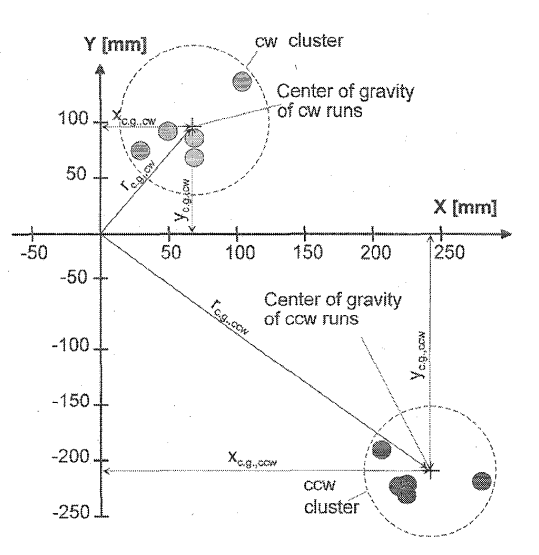
\includegraphics[scale=1]{image/umbmark_plot.png}
\caption{Typical results from UMBmark experiments}
\label{fig:data_plot}
\end{figure}

\textbf{Note:} You are expected to shoot videos for both the initial
version and the corrected version of your robot. Combining two videos in
a single video is encouraged. Also you can include only one run of the experiments.
 
\end{document}
